% ============================================================================
% Section: Robust Power-Share Controller Design
% Uses amsmath, graphicx, booktabs, siunitx (loaded in main file).
% All numeric values carry a % comment citing the source file under
% controller_design/. Prose marked % NOTE is placeholder for the human author.
% ============================================================================

\section{Robust Power-Share Controller Design}
\label{sec:robust}

% NOTE (author): opening paragraph is a placeholder skeleton -- rewrite to connect
% back to the EMS section and to state the thesis contribution in one sentence.
The energy-management supervisor running on the vehicle's companion computer emits a
requested power-share $\alpha_{req}\in[0,1]$ at up to \SI{50}{\hertz}. Realising that
request on hardware is the job of an inner loop that adjusts the analogue droop
resistance of each of the two boost converters until the measured current split matches
the request. This section derives the plant seen by that loop, argues why a
nominal-tuned PI controller is inadequate for it, synthesises a robust replacement by
$\mathcal{H}_\infty$ mixed-sensitivity design followed by a Youla parameterisation gain
adjustment, and validates the result against both a 60-corner uncertainty family and an
independently constructed full-order converter model.

% ---------------------------------------------------------------------------
\subsection{Plant Model of the Droop-Controlled Share Loop}
\label{sec:share-plant}

% NOTE(orchestrator): the droop chain derivation and Eq. (share law) also appear in
% Section \ref{sec:droop}. In the final paper keep the full derivation in Sec. 2 and
% reduce this subsection to the *dynamic* modeling (design plant, corners), citing
% back. Kept in full here so each section reads standalone during planning.

\subsubsection{Per-channel programmable output resistance}

Each source channel (fuel cell, FC; battery, BT) is a synchronous boost converter whose
output voltage is drooped in analogue hardware in proportion to its own output current.
The sensed current passes through a current-sense amplifier of gain
$K_{sns}=\SI{0.1}{\volt\per\ampere}$, % system_model.md §8 (INA253A1IPWR fitted, A1 variant)
a 12-bit multiplying DAC of programmable gain $g\in[0,1]$, and a non-inverting stage of
gain $A_v = 1 + R_{op2}/R_{op1} = \num{5.02}$, % system_model.md §2 (R_op1=10k, R_op2=40.2k)
and is then injected into the regulator feedback node through $R_{inj}=\SI{53.6}{\kilo\ohm}$
against the divider $R_{D1}=\SI{215}{\kilo\ohm}$, $R_{D2}=\SI{10}{\kilo\ohm}$.
% system_model.md §8: R_D1 bodged 237k -> 215k on both channels (16 V bus retune, 2026-07-11)
Applying Kirchhoff's current law at the feedback node, which the regulator servos to
$V_{ref}$, gives a Th\'evenin source with an \emph{electronically programmable} output
resistance

\begin{equation}
V_{out} = V_0 - R_e(g)\,I_{out},
\qquad
R_e(g) = K_{sns}A_v\frac{R_{D1}}{R_{inj}}\,g \;=\; R_{e,max}\,g .
\label{eq:Re-robust}
\end{equation}

With the fitted values, $R_{D1}/R_{inj}=\num{4.0112}$, $V_0 = \SI{15.91}{\volt}$ and
$R_{e,max} = \SI{2.014}{\ohm}$, % system_model.md §2 and §8 (derived: K_sns·A_v·R_D1/R_inj)
giving a droop resolution of \SI{0.492}{\milli\ohm} per DAC code.
% system_model.md §2: ΔR_e = R_e,max/4096

% NOTE (author): the sentence below records a firmware defect found by this modelling
% exercise. It is told at length in Section \ref{sec:droop:bug}; here it is only a
% cross-reference. Decide which section owns the story.
The factor $R_{D1}/R_{inj}$ --- the attenuation of the injection path by the feedback
divider --- was omitted in the original firmware droop mapping, which therefore commanded
DAC gains $g>1$ over almost the entire ratio range and left both DACs clamped at full
scale. The share loop consequently saw a \emph{zero-gain} plant, a defect invisible to
any nominal-model simulation and only exposed by writing~\eqref{eq:Re-robust} out against
the schematic (Section~\ref{sec:droop:bug}).

\subsubsection{Two channels in parallel: the static share law}

Both Th\'evenin sources feed the DC bus through ideal-diode switches. With
$V_{bus}=V_{0F}-R_FI_F=V_{0B}-R_BI_B$ and $I_F+I_B=I_{tot}$, and adopting the
droop-ratio mapping $R_F = k_d/r$, $R_B = k_d/(1-r)$ --- for which the parallel droop
$R_F\!\parallel\!R_B = k_d$ is independent of $r$ --- the measured share obeys

\begin{equation}
\alpha \;\equiv\; \frac{I_F}{I_{tot}}
\;=\; r \;+\; \underbrace{\frac{\Delta V_0\,r(1-r)}{k_d\,I_{tot}}}_{d},
\qquad \Delta V_0 \equiv V_{0F}-V_{0B}.
\label{eq:share-static}
\end{equation}

Three structural facts follow, and they set the entire control problem.

\begin{enumerate}
\item \textbf{The nominal static gain is exactly unity} ($\alpha=r$ when $\Delta V_0=0$),
by construction of the $k_d/r$ mapping. This is precisely why a PI controller with
$K_p=K_i=1$ appeared adequate on paper.
\item \textbf{Set-point mismatch enters as an additive output disturbance} $d$, worst at
$r=0.5$ and at light load, and inversely proportional to the droop scale $k_d$. With a
plausible per-board $\Delta V_0 = \SI{0.4}{\volt}$ and $k_d = \SI{0.30}{\ohm}$,
$d = 0.33/I_{tot}$, i.e.\ \textbf{0.17 share at \SI{2}{\ampere}}. % system_model.md §5a
This is a very large static offset and is the reason exact integral action is a hard
requirement rather than a refinement.
\item \textbf{The same mismatch perturbs the plant gain},
$\partial\alpha/\partial r = 1 + \Delta V_0(1-2r)/(k_d I_{tot})$, which is treated as
parametric gain uncertainty $K\in[1-\delta,1+\delta]$.
\end{enumerate}

The actuator constraint $g\le 1$ bounds the usable authority:
$k_d \le R_{e,max}\min(r_{min},1-r_{max})$. The design adopts
$r\in[\num{0.15},\num{0.85}]$ with $k_d=\SI{0.30}{\ohm}$ (hard bound \SI{0.3020}{\ohm}),
% system_model.md §4 trade table
which trades a \SI{1.8}{\volt} bus sag at \SI{6}{\ampere} against a manageable mismatch
disturbance. Twelve-bit DAC quantisation moves the share by $\approx\num{3.7e-5}$ per
code at the range edge and is negligible against the sensor noise floor.
% system_model.md §4 quantization paragraph

\subsubsection{Dynamics and the design plant}

The share statics are, remarkably, \emph{instantaneous}: with $\Delta V_0=0$ both channel
currents carry the common factor $(V_0-V_{bus}(t))$, so
$\alpha(t) = G_F/(G_F+G_B) = r$ at every instant regardless of the bus-voltage transient.
% system_model.md §6a
The bus-capacitance pole therefore appears in the share response only through the
mismatch term, with residue $\propto \Delta V_0/(k_dI_{tot})$, and is absorbed into the
uncertainty description rather than modelled explicitly. What remains is the digital
layer plus the converter voltage loops, giving the design plant

\begin{equation}
G_P(s) \;=\; \frac{K\,e^{-T_d s}}{(\tau_r s + 1)(\tau_f s + 1)} .
\label{eq:design-plant}
\end{equation}

\begin{table}[H]
\caption{Design-plant parameters and uncertainty ranges.}
\label{tab:plant-params}
\begin{tabular}{llll}
\toprule
\textbf{Parameter} & \textbf{Nominal} & \textbf{Range} & \textbf{Physical origin}\\
\midrule
$K$      & 1                  & $[0.55,\ 1.45]$          & static mismatch gain term, Eq.~\eqref{eq:share-static}\\
$T_d$    & \SI{1.0}{\milli\second} & $[0.5,\ 2.0]$~ms    & zero-order hold $+$ compute-to-apply latency at $T_s=\SI{1}{\milli\second}$\\
$\tau_r$ & \SI{100}{\micro\second} & $[20,\ 300]$~\textmu s & converter voltage-loop lag, lumped with sense and bus parasitics\\
$\tau_f$ & \SI{0.8}{\milli\second} & $\{0,\ 0.8\}$~ms    & optional \SI{200}{\hertz} measurement prefilter\\
\bottomrule
\end{tabular}
\end{table}
% Table values: system_model.md §6d. Wide K set [0.55,1.45] applies at the r-range edges
% with the full ±0.4 V mismatch budget; [0.75,1.25] holds for r∈[0.3,0.7] at I_tot ≥ 2 A.

The loop delay budget is $T_d = T_s/2 + T_s + \varepsilon \approx \SI{1.5}{\milli\second}$
worst case at the chosen \SI{1}{\kilo\hertz} rate, which gives $\ge 20\times$
oversampling of the intended \SIrange{5}{10}{\hertz} closed-loop bandwidth while leaving
the fast firmware tick free for fault detection and motor control.
% system_model.md §6c

The plant is thus \emph{delay-dominated with near-unity gain}. The lumping of the two
converter voltage loops into the single lag $\tau_r$ is justified by time-scale
separation of about \num{2.5} decades: the converter loops cross at
\SIrange{6}{22}{\kilo\hertz} (from datasheet compensator arithmetic with
$R_C=\SI{61.2}{\kilo\ohm}$ on \emph{both} channels), % system_model.md §6e
whereas the share loop crosses near \SI{110}{\radian\per\second}. Even the slowest
modelled $\tau_r=\SI{300}{\micro\second}$ contributes only $\ang{1.9}$ of phase at the
share crossover. Section~\ref{sec:fullorder} replaces this argument with empirical
evidence.

% ---------------------------------------------------------------------------
\subsection{Why Robustness, and Not Tuning, Is the Issue}
\label{sec:why-robust}

% NOTE (author): this subsection carries the paper's argument. Rewrite the prose freely,
% but keep the 26.9 vs 1.87 comparison as the headline claim -- it is the single number
% that justifies the whole design effort.
Equation~\eqref{eq:share-static} makes the plant look trivial: unity DC gain, one small
lag, one small delay. That appearance is exactly the trap. The unity gain is a property
of the \emph{nominal} hardware, and the two channels are not nominally identical in
practice:

\begin{itemize}
\item \textbf{Regulator tolerance bands are wide.} The converter feedback reference is
specified over \SIrange{0.588}{0.612}{\volt} across process and temperature ($\pm\SI{2}{\percent}$),
% system_model.md §5a, TPS61288LRQQR.pdf §7.5
and with $\pm\SI{1}{\percent}$ divider resistors the channel-to-channel no-load voltage
difference budgets to $\pm\SI{3.4}{\percent}$, i.e.\ $\Delta V_0 \approx \pm\SI{0.6}{\volt}$
worst case. Through Eq.~\eqref{eq:share-static} this is simultaneously a large output
disturbance \emph{and} a plant-gain perturbation.
\item \textbf{Ceramic output capacitance derates strongly with bias.} The three
\SI{22}{\micro\farad} output capacitors present \SI{66}{\micro\farad} nominally but
$\approx\SI{30}{\micro\farad}$ derated, % full_order_validation.md §3 envelope axes
which moves each converter's voltage-loop crossover by better than a factor of two and
hence moves $\tau_r$.
\item \textbf{The right-half-plane zero moves with load and duty.} $f_{RHPZ}$ ranges over
\SIrange{31}{330}{\kilo\hertz} across the \SIrange{2}{8}{\ampere} load envelope,
% system_model.md §6e item 2
so the converter dynamics that the lump is meant to cover are themselves operating-point
dependent.
\item \textbf{The channels are asymmetric by construction.} They run from different input
voltages (\SIrange{9}{12}{\volt} fuel-cell side versus \SIrange{7.4}{8.4}{\volt} battery
side), % system_model.md §6e table
so their duty cycles, RHP zeros and crossovers differ even with identical components.
Matching the compensator resistor across the two channels was a deliberate hardware
change made \emph{so that} a single shared $\tau_r$ would be defensible.
\item \textbf{Measurement noise scales as $1/I_{tot}$.} One ADC code is
\SI{8.06}{\milli\ampere}, % system_model.md §5b (SCALE_I)
so the share measurement quantises at \SI{0.4}{\percent} at \SI{2}{\ampere} but
\SI{1.6}{\percent} at \SI{0.5}{\ampere}, requiring high-frequency roll-off of the actuator
signal to avoid DAC chatter.
\end{itemize}

A controller tuned at the nominal point cannot be assumed to survive this set, and in
this case it does not. Evaluated on the discrete closed loop over the parameter corners
of Table~\ref{tab:plant-params}, the legacy $K_p=K_i=1$ PI reaches a peak sensitivity of
$\|S\|_\infty = \num{26.9}$ (\SI{28.6}{\decibel}), whereas the robust design developed
below peaks at $\|S\|_\infty = \num{1.87}$ (\SI{5.4}{\decibel}).
% synthesis_metrics.txt: "discrete worst ||S||inf: youla = 1.867, legacy PI = 26.889"
A sensitivity peak of \num{26.9} corresponds to a disk margin so small that the loop is,
for engineering purposes, conditionally stable at the corners --- and the corners here
are not exotic: they are a cold board, a derated capacitor, and two converters from
different reels. This factor-of-\num{14} gap in worst-case sensitivity peak, not any
improvement in nominal step response, is the justification for a robust synthesis.

% ---------------------------------------------------------------------------
\subsection{\texorpdfstring{$\mathcal{H}_\infty$}{H-infinity} Synthesis and Youla-H Gain Adjustment}
\label{sec:synthesis}

\subsubsection{Mixed-sensitivity problem and weight selection}

The controller is synthesised by mixed-sensitivity $\mathcal{H}_\infty$ design on the
stacked $S/KS/T$ problem, followed by the Youla-H post-synthesis gain adjustment of
Tan et~al.\ that enforces exact unity DC complementary sensitivity.
% controller_synthesis.md header: method = Tan, Yadav, Assadian 2026
The delay is represented by a second-order Pad\'e approximant, so the nominal augmented
plant has four states.

\begin{table}[H]
\caption{Synthesis weights and their design intent.}
\label{tab:weights}
\begin{tabular}{llll}
\toprule
\textbf{Weight} & \textbf{Acts on} & \textbf{Form / values} & \textbf{Intent}\\
\midrule
$W_p$ & $S$ & strictly proper $Ma/(s+a)$, $M=10^4$, unity crossing \SI{40}{\radian\per\second} & integral-action pressure; disturbance rejection below \SI{40}{\radian\per\second}\\
$W_d$ & $T$ & \texttt{makeweight(0.5, 250, 40)} & force $T$ roll-off above \SI{250}{\radian\per\second} (noise, unmodelled HF)\\
$W_u$ & $Y$ & \texttt{makeweight(0.3, 600, 20)} & cap actuator effort; roll off DAC activity above \SI{600}{\radian\per\second}\\
\bottomrule
\end{tabular}
\end{table}
% Weight table: controller_synthesis.md §2

$W_p$ is deliberately chosen \emph{strictly} proper. Since $S\to 1$ at high frequency
needs no penalty, this costs nothing in design terms but makes the augmented plant
satisfy $D_{11}=0$ exactly, so the regular DGKF problem applies and the estimation
Riccati equation degenerates analytically ($D_{21}=1 \Rightarrow Q_y=0$, $A-B_1C_2$
stable $\Rightarrow Y=0$), leaving a single Riccati solve and the central controller
$\dot{\hat{x}} = (A-B_1C_2+B_2F)\hat{x} + B_1e$, $u=F\hat{x}$.
% controller_synthesis.md §1
% NOTE (author): the following sentence is a methods disclosure -- keep or cut depending
% on whether the venue wants reproducibility detail at this level.
Because no commercial robust-control toolbox was available on the development machine,
the Riccati solutions were computed from the Hamiltonian matrix by ordered real Schur
decomposition with $\gamma$-iteration by bisection, in a purpose-written implementation
whose primitives are unit-tested against reference solvers and whose every synthesised
controller passes an \emph{a-posteriori} gate: closed-loop stability plus
$\|T_{zw}\|_\infty \le \gamma$ evaluated by an independent Hamiltonian-bisection norm.
A derivation error therefore cannot silently yield an accepted controller.

\subsubsection{Synthesis result and the \texorpdfstring{$T(0)=1$}{T(0)=1} step}

\begin{table}[H]
\caption{Synthesis outcome (nominal plant).}
\label{tab:synth-results}
\begin{tabular}{ll}
\toprule
\textbf{Quantity} & \textbf{Value}\\
\midrule
$\gamma_{opt}$                                 & \num{0.6532}\\          % synthesis_metrics.txt
Controller built at                            & $\gamma=\num{0.6859}$ (\SI{5}{\percent} back-off), $\|T_{zw}\|_\infty=\num{0.6841}$ \checkmark\\ % synthesis_metrics.txt
$\mathcal{H}_\infty$ controller order          & 7 (4 plant $+$ 3 weight states)\\ % controller_synthesis.md §3
$T_H(0)$ before adjustment                     & \num{0.99996423}\\      % synthesis_metrics.txt
$T_{YH}(0)$ after adjustment                   & \num{1.000000000000}\\  % synthesis_metrics.txt
$S/T$ crossover                                & \SI{109.9}{\radian\per\second}\\ % synthesis_metrics.txt
$\|S\|_\infty,\ \|T\|_\infty,\ \|Y\|_\infty$   & \num{1.25}, \num{1.00}, \num{1.01}\\ % controller_synthesis.md §3
Nominal $M_2$ / phase margin / delay margin    & \num{0.7978} / \ang{73.9} / \SI{11.74}{\milli\second}\\ % synthesis_metrics.txt
\bottomrule
\end{tabular}
\end{table}

That $\gamma_{opt}<1$ with margin means every weighted specification is met, but the
$\mathcal{H}_\infty$ solution exhibits the classical DC deficiency: $T_H(0)=\num{0.99996423}$,
short of unity by \SI{0.0036}{\percent}. For this application that residual is not
cosmetic. It leaves a finite DC loop gain, so the static mismatch disturbance $d$ of
Eq.~\eqref{eq:share-static} --- which can be \num{0.17} in share at \SI{2}{\ampere} --- is
only attenuated, not rejected, and a ramping EMS reference accrues a persistent bias.

The Youla-H step applies the scalar gain correction $Y_{YH} = Y_H/T_H(0)$ and recovers
the controller as $G_{C,YH} = Y_{YH}(1-G_PY_{YH})^{-1}$.
% controller_synthesis.md §3
This \SI{+0.0036}{\percent} gain shift places an exact integrator in the controller: the
near-origin pole of $G_{C,YH}$ appears at $|p|=\num{5.6e-9}$ and is snapped to a true
integrator by the spectral split of the following subsection. The outcome is
$T(0)=1$ to machine precision, hence exact DC disturbance rejection and zero ramp-following
bias, obtained \emph{without} re-tuning the weights and without disturbing the
$\mathcal{H}_\infty$ robustness the synthesis just bought.

\begin{figure}[H]
\centering
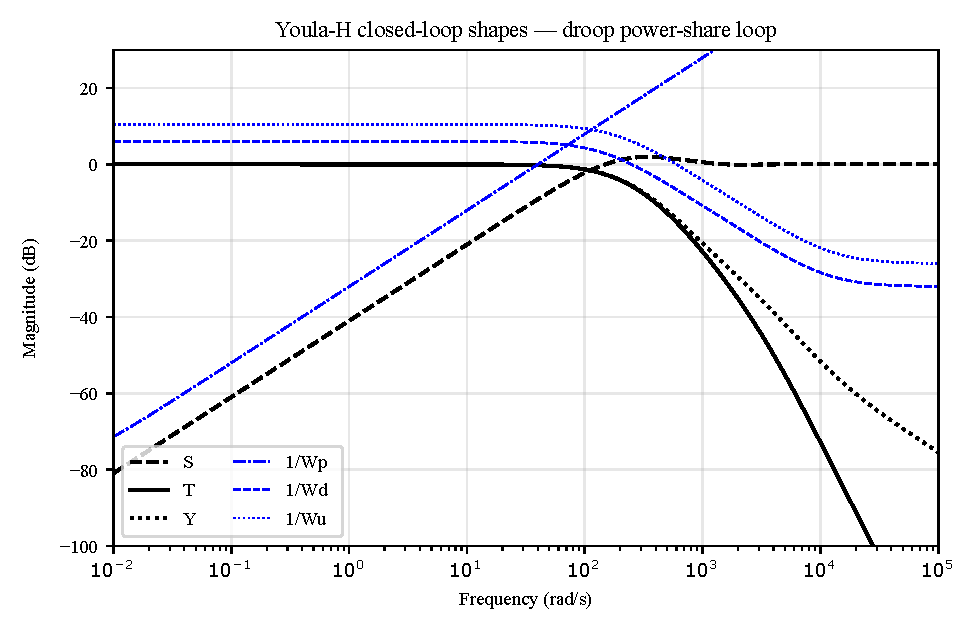
\includegraphics[width=\textwidth]{Figures/loopshapes_youla_h.pdf}
% source: controller_design/figures/loopshapes_youla_h.svg (data: loopshapes_youla_h.csv)
\caption{Achieved sensitivity $S$, complementary sensitivity $T$ and control sensitivity
$Y$ of the Youla-H design, plotted against the inverse weights $1/W_p$, $1/W_d$, $1/W_u$.
All three lie inside their templates, consistent with $\gamma_{opt}=\num{0.6532}$.}
\label{fig:loopshapes}
\end{figure}

\subsubsection{Order reduction, discretisation, and firmware realisation}

The controller is decomposed as $G_{C,YH}(s) = k_I/s + R(s)$ with
$k_I=\num{111.93}$ % synthesis_metrics.txt: kI = 111.929630
--- consistent with the observed crossover, since $|L|=1$ where $k_I/\omega\approx 1$ ---
and the 21-state stable remainder $R(s)$ is reduced by balanced truncation to
\textbf{three states}. The Hankel singular values (\num{14.8}, \num{0.035}, \num{0.0018},
\num{5e-5},~\ldots) % controller_synthesis.md §4
justify the cut, and the reduced controller's frequency response deviates from the full
one by at most \SI{0.8}{\percent}.

Tustin discretisation at $T_s=\SI{1}{\milli\second}$ yields three second-order sections
plus a trapezoidal integrator. The embedded implementation evaluates

\begin{equation}
u_k = r_0 + R(z)e_k + I(z)e_k, \qquad r_0 = 0.5,
\qquad r_k = \mathrm{sat}_{[r_{min},\,r_{max}]}(u_k),
\label{eq:ctrl-impl}
\end{equation}

as a cascade of Direct-Form-II-transposed biquads in single precision, with the output
clamped to $[\num{0.15},\num{0.85}]$. Anti-windup is by \textbf{back-calculation on the
output clamp}: when $u_k$ would leave the interval, the integrator state absorbs exactly
the excess, so the command sits on the rail and resumes moving on the tick the error
reverses. The biquad states are deliberately \emph{not} clamped --- $R(z)$ is stable and
cannot wind up, so clamping it would only introduce a spurious nonlinearity. The measured
share (only --- never the set-point) passes through the \SI{200}{\hertz} one-pole
prefilter that is part of the design plant as $\tau_f$, so EMS steps are not smoothed by
a sensor filter. A wrapper gates the update to exactly one execution per $T_s$ and holds
the output between ticks; that zero-order hold is itself accounted for in $T_d$.

Two implementation notes are worth recording. First, one discrete section carries a pole
at $z=\num{0.999996}$ --- the $W_p$ weight pole reappearing nearly cancelled in the
controller. Its distance from the unit circle, \num{4e-6}, is about $30\times$ single-
precision epsilon at unity, so the section is representable, and its Hankel singular value
(\num{0.035}) shows it genuinely contributes rather than being truncation noise.
% controller_synthesis.md §4 and §8
Second, the loop freezes (states held, no integration) when $I_{tot}\approx 0$, matching
the validity limit of Eq.~\eqref{eq:share-static}, where $\alpha$ is undefined.

\begin{figure}[H]
\centering
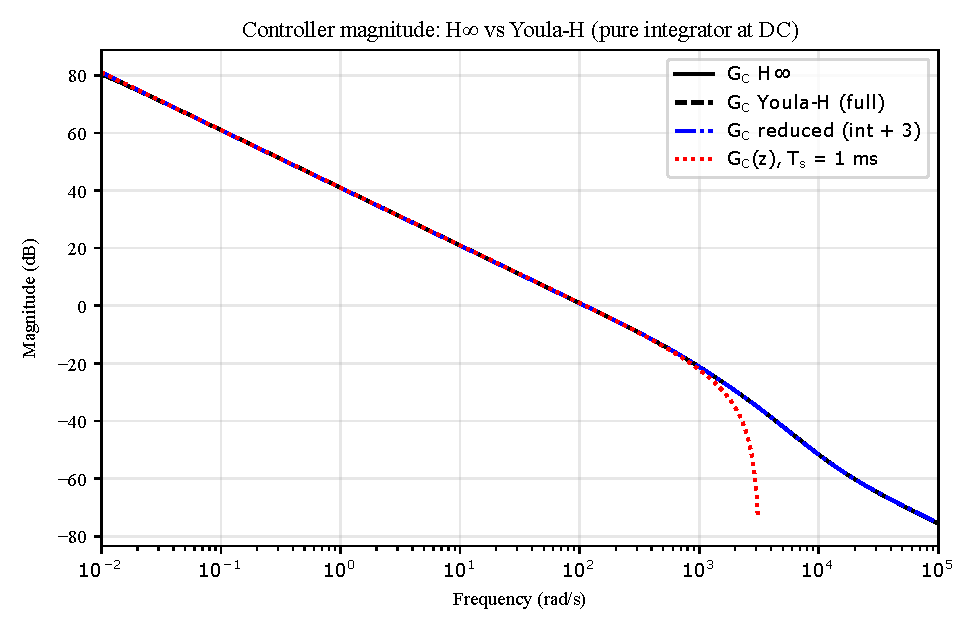
\includegraphics[width=\textwidth]{Figures/controller_bode.pdf}
% source: controller_design/figures/controller_bode.svg (data: controller_bode.csv)
\caption{Controller frequency response at each stage of the realisation: the raw
$\mathcal{H}_\infty$ controller, the Youla-H adjusted controller, the reduced
form, and the discretised implementation. The exact integrator introduced by
the Youla-H step is visible as the diverging low-frequency branch that the raw
$\mathcal{H}_\infty$ controller lacks.}
\label{fig:ctrl-bode}
\end{figure}

% ---------------------------------------------------------------------------
\subsection{Validation}
\label{sec:validation}

\subsubsection{Corner sweeps and time-domain behaviour}

The design was checked over the full uncertainty family of Table~\ref{tab:plant-params}:
$K\in\{0.55\ldots1.45\}$, $T_d\in\{0.5,1,2\}$~ms, $\tau_r\in\{20,300\}$~\textmu s,
$\tau_f\in\{0,0.8\}$~ms, i.e.\ \textbf{60 corners}. All 60 continuous-time closed loops
are stable, with worst-case $M_2=\num{0.5905}$ occurring at $(K,T_d,\tau_r,\tau_f) =
(\num{1.45}, \SI{2}{\milli\second}, \SI{300}{\micro\second}, \SI{0.8}{\milli\second})$;
% synthesis_metrics.txt: worst-corner M2 = 0.5905 at (1.45, 0.002, 0.0003, 0.0008)
the corresponding discrete sweep (zero-order-hold plant against the \emph{implemented}
$G_C(z)$) has all closed-loop poles inside the unit circle.

\begin{table}[H]
\caption{Validation summary. All entries generated by the synthesis pipeline.}
\label{tab:validation}
\begin{tabular}{lll}
\toprule
\textbf{Check} & \textbf{Result} & \textbf{Source}\\
\midrule
Continuous 60-corner sweep      & all stable, worst $M_2=\num{0.5905}$          & \texttt{synthesis\_metrics.txt}\\
Discrete 60-corner sweep        & all $|z|<1$                                    & \texttt{synthesis\_metrics.txt}\\
Nominal margins                 & GM \SI{18.5}{\decibel}, PM \ang{73.9} at \SI{110}{\radian\per\second}, delay margin \SI{11.74}{\milli\second} & \texttt{MATLAB\_validation.txt}\\
Step $0.5\to0.7$ (discrete)     & \SI{2}{\percent} settle \SI{22}{\milli\second}, \SI{0}{\percent} overshoot, SS error \num{8e-9} & \texttt{synthesis\_metrics.txt}\\
Ramp \SI{0.05}{\per\second}     & tracking error \num{4.47e-4}, no accumulating bias & \texttt{synthesis\_metrics.txt}\\
Anti-windup (\SI{0.5}{\second} into the rail) & leaves rail $\le 3$ ticks after error reversal, recovery $<\SI{150}{\milli\second}$ & \texttt{controller\_synthesis.md} §5\\
Worst-corner discrete $\|S\|_\infty$ & \textbf{\num{1.867}} (legacy PI: \num{26.889}) & \texttt{synthesis\_metrics.txt}\\
\bottomrule
\end{tabular}
\end{table}

The delay margin of \SI{11.74}{\milli\second} deserves emphasis: it is roughly
$6\times$ the worst \emph{modelled} loop delay of \SI{2}{\milli\second}. Since the timing
parameters are pre-calibration estimates, this margin --- not any single nominal number
--- is what makes the design safe to commit to firmware ahead of bench identification.

\begin{figure}[H]
\centering
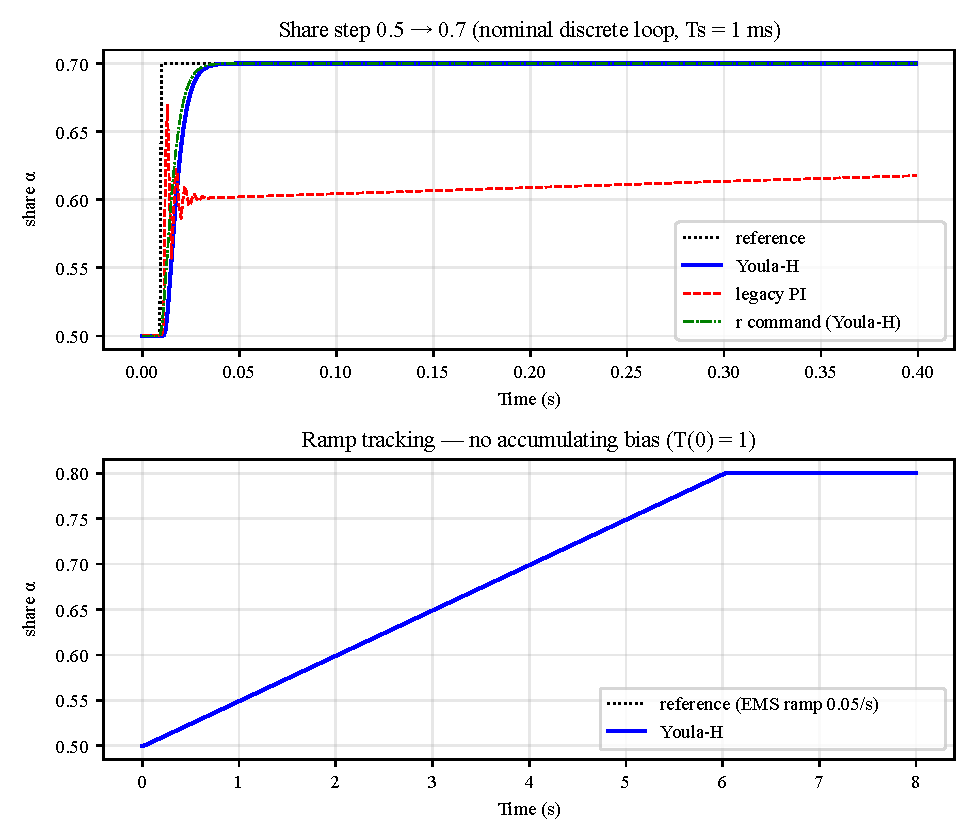
\includegraphics[width=\textwidth]{Figures/timedomain_step_ramp.pdf}
% source: controller_design/figures/timedomain_step_ramp.svg (data: timedomain_step_ramp.csv)
\caption{Discrete-time closed-loop response of the implemented controller: share step
$0.5\to0.7$ (left) and ramp reference at \SI{0.05}{\per\second} (right). The ramp
panel is the practical expression of $T(0)=1$: the tracking error decays to
\num{4.5e-4} instead of settling to a constant offset.}
\label{fig:timedomain}
\end{figure}

\begin{figure}[H]
\centering
% TODO(figure): no rendered figure exists yet — plot from
% controller_design/figures/step_response_nominal.csv and step_response_mismatch.csv
% (columns: t_s, r_cmd, alpha, v_bus).
\fbox{\parbox[c][4cm][c]{0.9\textwidth}{\centering PLACEHOLDER --- plot from
\texttt{step\_response\_nominal.csv} / \texttt{step\_response\_mismatch.csv}}}
\caption{Open-loop verification of the static share law, Eq.~\eqref{eq:share-static},
from the independent numerical model: commanded ratio $r$, achieved share $\alpha$, and
bus voltage. With matched channels ($\Delta V_0 = 0$) the share tracks $r$ instantaneously;
the companion mismatch case ($\alpha = \num{0.48}$ at $r = \num{0.40}$) shows the
open-loop offset that only integral action can remove.}
\label{fig:step-openloop}
\end{figure}

\subsubsection{Full-order cross-validation}
\label{sec:fullorder}

The design plant~\eqref{eq:design-plant} rests on lumping two converter voltage loops into
one uncertain lag. To test that reduction rather than merely argue it, a complete
small-signal model of the share plant was constructed \emph{independently}: both channels'
transconductance-amplifier compensators with the exact COMP-node impedance
$Z_{comp}=R_{EA}\|(R_C+1/sC_C)\|1/sC_P$, Norton-equivalent power stages carrying the
right-half-plane and ESR zeros, the three-resistor feedback node with the bilinear droop
injection linearised at $(g_0,I_0)$, current-sense dynamics, bus coupling, and the same
digital layer --- \textbf{11 states} per operating point, against two states plus a delay
in the design model.
% full_order_validation.md §1.1-1.4

Structural gate checks confirm the construction before any comparison is drawn: the
Norton form reduces to the datasheet power-stage expression to machine precision
($\num{4.5e-16}$); the DC share gain emerging from the full linearisation is \num{0.9933},
short of unity only by the finite error-amplifier DC gain; and the per-channel voltage-loop
crossovers reproduce the independent datasheet arithmetic to within \SIrange{1}{3}{\percent}
(e.g.\ FC \SI{16.33}{\kilo\hertz} computed versus \SI{16.84}{\kilo\hertz} predicted).
% full_order_validation.md §2, gates A/B/C

\begin{table}[H]
\caption{Full-order versus simplified plant, and closed-loop equivalence with the shipped
controller.}
\label{tab:fullorder}
\begin{tabular}{lll}
\toprule
\textbf{Check} & \textbf{Full-order model} & \textbf{Simplified model}\\
\midrule
Nominal in-band deviation ($\omega\le\SI{1100}{\radian\per\second}$) & \SI{3.86}{\percent} & --- \\
Envelope deviation, 432 operating points & \SI{5.78}{\percent} worst, \SI{4.30}{\percent} median & ---\\
Discrete closed-loop stability & \textbf{432/432} points & 60/60 corners\\
Worst discrete $\|S\|_\infty$ & \textbf{\num{1.240}} & \num{1.867}\\
Step $0.5\to0.7$ overlay & max divergence \num{0.0008} share & ---\\
\SI{2}{\percent} settle & \SI{25}{\milli\second} & \SI{22}{\milli\second}\\
Ramp error at \SI{3}{\second} & \num{4.30e-4} & \num{4.47e-4}\\
\bottomrule
\end{tabular}
\end{table}
% All entries: fullorder_metrics.txt

The 432-point envelope spans $\{V_{in,FC}\;9/12\}\times\{V_{in,BT}\;7.4/8.4\}\times
\{I_{tot}\;1/2/4\,\mathrm{A}\}\times\{r_0\;0.3/0.5/0.7\}\times\{C_O\;30/66\,\mu\mathrm{F}\}
\times\{C_{bus}\;30/500\,\mu\mathrm{F}\}\times\{R_{EA}\;1/10/100\,\mathrm{M}\Omega\}$;
% full_order_validation.md §3
the amplifier output resistance is swept rather than assumed because the datasheet does
not specify it, converting a hidden assumption into a verified non-sensitivity.

Two results matter. First, every full-order response lies within \SI{5.78}{\percent} of
\emph{some} member of the simplified corner family, so the uncertainty set used for
synthesis was a genuine superset of the true dynamics. Second, the worst full-order
closed-loop sensitivity peak (\num{1.240}) is \emph{lower} than the simplified family's
worst (\num{1.867}) --- the expected sign, confirming that the corner family was
pessimistic in the safe direction rather than accidentally optimistic in some unmodelled
one.

\begin{figure}[H]
\centering
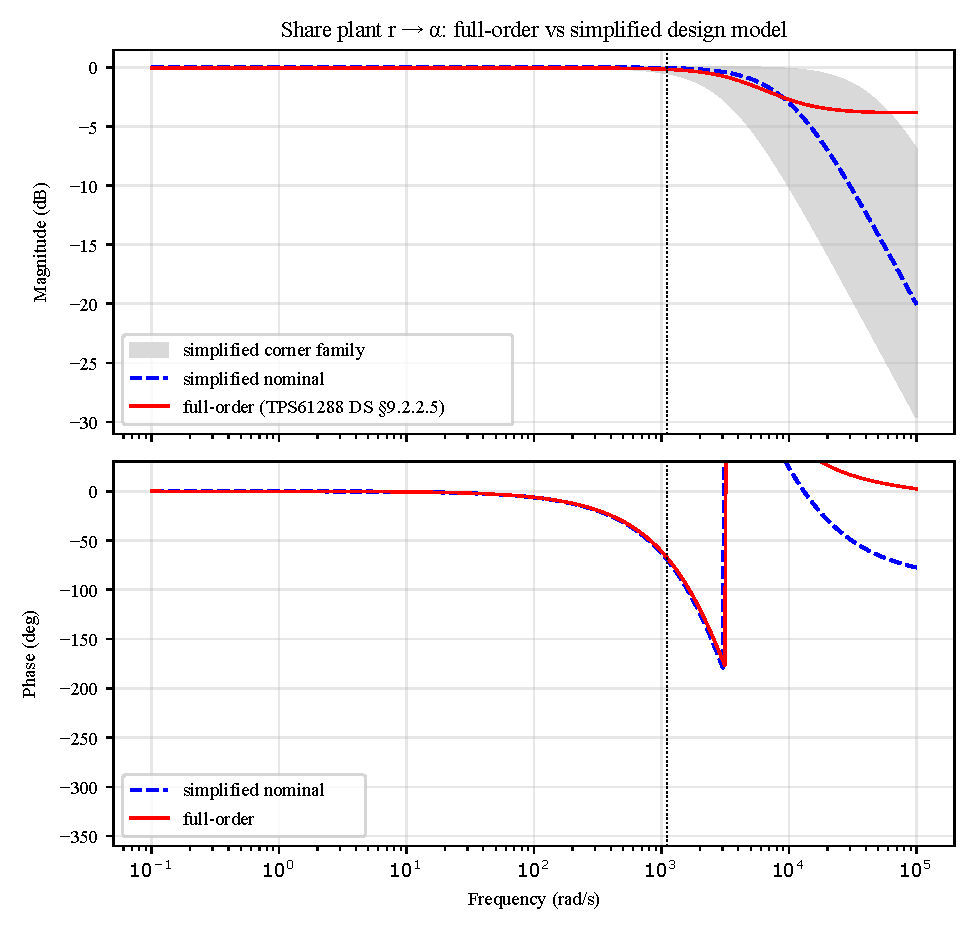
\includegraphics[width=\textwidth]{Figures/fullorder_bode_overlay.pdf}
% source: controller_design/figures/fullorder_bode_overlay.svg (data: fullorder_bode_overlay.csv)
\caption{Nominal open-loop frequency response of the 11-state full-order model overlaid on
the two-state-plus-delay design plant. The traces are visually indistinguishable through
the design band ($\omega\le\SI{1100}{\radian\per\second}$, max deviation \SI{3.86}{\percent})
and separate only beyond $\approx\SI{e4}{\radian\per\second}$, where the share-loop gain is
far below unity.}
\label{fig:fo-bode}
\end{figure}

\begin{figure}[H]
\centering
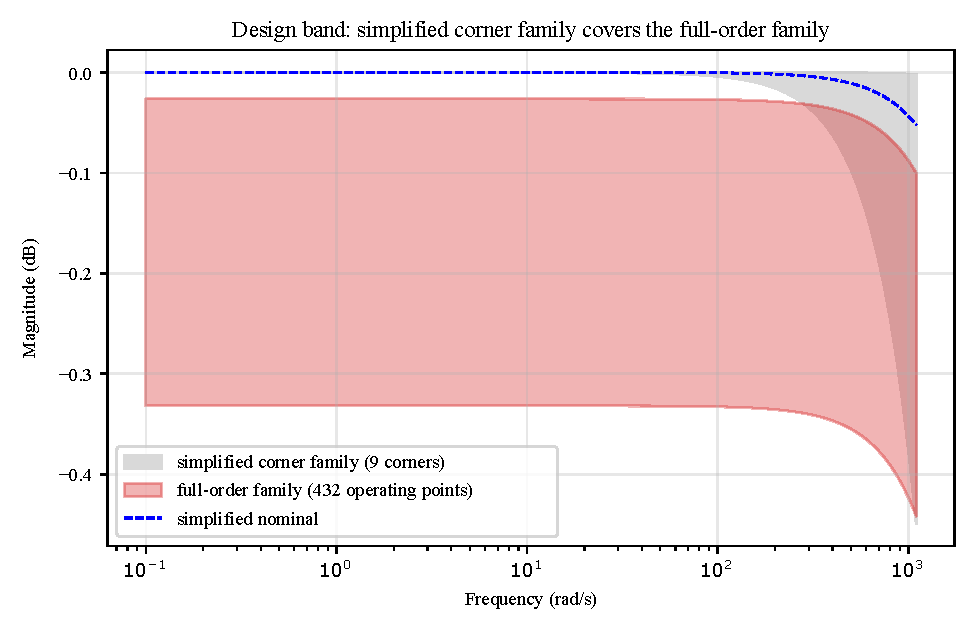
\includegraphics[width=\textwidth]{Figures/fullorder_envelope.pdf}
% source: controller_design/figures/fullorder_envelope.svg (data: fullorder_envelope.csv)
\caption{Envelope study: 432 full-order operating points against the simplified corner
family. The corner family bounds the full-order family with margin, which is the condition
for the synthesis uncertainty set to be valid.}
\label{fig:fo-envelope}
\end{figure}

\begin{figure}[H]
\centering
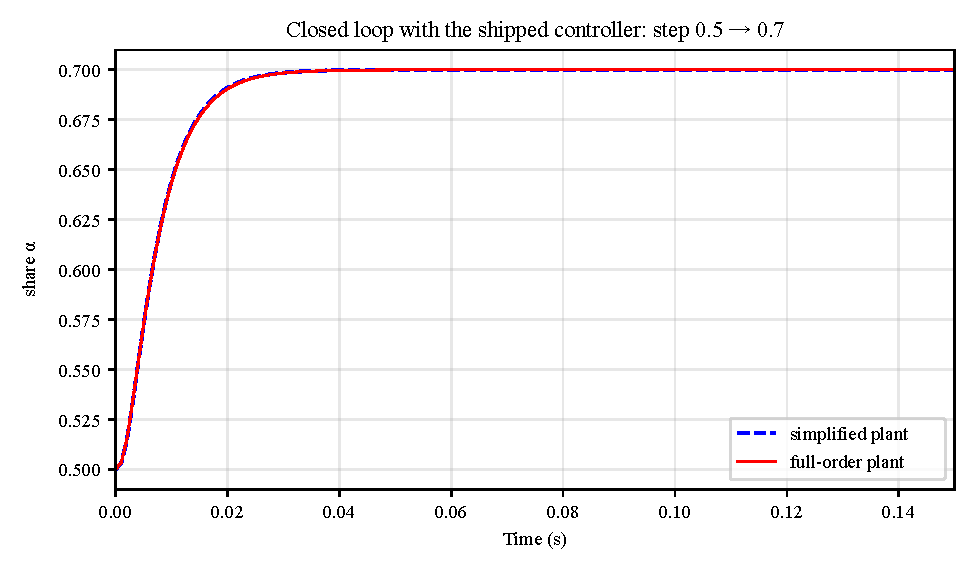
\includegraphics[width=\textwidth]{Figures/fullorder_step_overlay.pdf}
% source: controller_design/figures/fullorder_step_overlay.svg (data: fullorder_step_overlay.csv)
\caption{Closed-loop step response of the shipped controller on the full-order plant
overlaid on the design prediction. Maximum divergence is \num{0.0008} share.}
\label{fig:fo-step}
\end{figure}

\subsubsection{Independent toolchain cross-check}

Because the synthesis was performed in a purpose-written solver, the entire result was
re-derived in a commercial robust-control toolbox using the same weights, and the
\emph{shipped} coefficients --- parsed directly from the firmware header rather than
re-synthesised --- were re-run through the validation battery in the firmware-accurate
loop topology.

\begin{table}[H]
\caption{Independent toolbox cross-check of the shipped controller.}
\label{tab:matlab}
\begin{tabular}{lll}
\toprule
\textbf{Quantity} & \textbf{Independent toolbox} & \textbf{Design pipeline}\\
\midrule
$\gamma_{opt}$              & \num{0.6553}      & \num{0.6532} ($+\SI{0.3}{\percent}$)\\
$T_H(0)$                    & \num{0.99996378}  & \num{0.99996423}\\
$k_I$                       & \num{110.429}     & \num{111.930} ($+\SI{1.36}{\percent}$)\\
Crossover                   & \SI{109.4}{\radian\per\second} & \SI{109.9}{\radian\per\second}\\
Nominal $M_2$               & \num{0.796}       & \num{0.798}\\
Corner sweep                & 30/30 stable, worst $\|S\|_\infty=\num{1.768}$ & 60/60 stable, worst \num{1.867}\\
Step / DC gain              & \SI{25}{\milli\second} settle, DC gain \num{1.000000001} & \SI{22}{\milli\second} settle\\
\bottomrule
\end{tabular}
\end{table}
% All entries: MATLAB_validation.txt (VERDICT: PASS)

The two independent syntheses agree on $\gamma_{opt}$ to \SI{0.3}{\percent} and on the
nominal margins to within measurement resolution; the \SI{9.5}{\percent} frequency-response
deviation between the shipped and re-synthesised controllers is attributable to the
$21\to3$ order reduction plus two independent $\gamma$-iterations, and the meaningful
comparison --- closed-loop behaviour and corner stability --- agrees closely.
% MATLAB_validation.txt section B note

% ---------------------------------------------------------------------------
\subsection{Limitations}
\label{sec:share-limitations}

% NOTE (author): keep this subsection. Reviewers reward stated limitations, and every item
% here is genuinely open at time of writing.
Three qualifications bound the claims above. First, the plant timing parameters
($T_d$, $\tau_r$, $C_{bus}$, $\Delta V_0$ and the droop scale $k_d$) are pre-calibration
estimates; the corner sweep is the hedge, and the design is deliberately delay-tolerant
(\SI{11.7}{\milli\second} margin against \SI{2}{\milli\second} worst modelled). A bench
identification procedure --- open-loop $r$-sweep to fit $\Delta V_0$ and confirm unity
slope, plus a step test on the current-sense outputs to extract $\tau_r$ and the true
$T_d$ --- is defined, after which the coefficients are regenerated through the same
automated pipeline. Second, the plant gain is assumed positive over the operating set;
below about \SI{1}{\ampere} total current with worst-case mismatch the gain envelope
widens beyond the design set, so the supervisor must avoid commanding extreme shares at
near-zero load (the loop is in any case frozen as $I_{tot}\to 0$). Third, the analysis is
small-signal and continuous-conduction; pulse-frequency-mode operation at light load is
unmodelled, though even a \SI{1}{\milli\second} effective lag would cost only \ang{6.3} at
the share crossover, less than the phase already budgeted by the \SI{2}{\milli\second}
delay corner.

% ============================================================================
% PLANNING NOTES
% ============================================================================
% 1. FIGURE FILES. All figure sources exist as SVG in controller_design/figures/:
%      loopshapes_youla_h.svg, controller_bode.svg, timedomain_step_ramp.svg,
%      fullorder_bode_overlay.svg, fullorder_envelope.svg, fullorder_step_overlay.svg,
%      droop_signal_chain.svg, control_loop_model.svg
%    Each has a matching .csv of raw data. step_response_nominal.csv and
%    step_response_mismatch.csv have NO rendered figure yet -- Fig.~\ref{fig:step-openloop}
%    must be plotted from the CSVs (columns: t_s, r_cmd, alpha, v_bus) before submission.
%    MDPI wants PDF/EPS, not SVG: convert with inkscape/cairosvg into Figures/ and keep
%    the .pdf extension used in the \includegraphics calls above.
%
% 2. NUMERIC DRIFT WARNING. Several constants were retuned on 2026-07-11 (16 V bus
%    retune: R_D1 237k -> 215k, hence R_e,max 2.220 -> 2.014 Ohm, V_0 15.91 V,
%    k_d 0.33 -> 0.30 Ohm). This section uses the POST-retune values from
%    system_model.md. Older project notes still quote the pre-retune numbers -- do not
%    mix them. If bench calibration lands before submission, EVERY number in the
%    tables here changes: regenerate via synthesize_controller.py ->
%    tps61288_full_model.py -> droop_plant.m and re-extract from the generated
%    *_metrics.txt files rather than editing by hand.
%
% 3. CITATIONS TO ADD. The method reference (Tan, Yadav, Assadian, "A Practical
%    Youla Gain-Tuning Framework for H-infinity Controller Realization" — the
%    companion paper in papers/A_Practical_Youla_Gain_Tuning_Framework...) is cited in
%    prose but has no \cite key yet. Also needs: DGKF 1989 for the central-controller
%    formulation, a standard reference for balanced truncation, and datasheet citations
%    for the boost converter, current-sense amplifier and multiplying DAC. Part numbers
%    have been kept out of the prose deliberately -- decide whether the venue wants them
%    named or kept generic, and apply consistently.
%
% 4. SECTION LENGTH. As drafted this runs long for a single Energies section
%    (~8 figures, 6 tables). Candidate cuts if space is tight:
%      - fold the validation summary + MATLAB cross-check tables into one;
%      - move the full-order validation to an appendix, keeping only the
%        two headline numbers (<6% deviation, 432/432 stable) in the main text;
%      - drop Fig. fullorder_envelope, which is the least self-explanatory plot.
%    Do NOT cut the 26.9 vs 1.87 comparison or the T(0)=1 argument -- those are the
%    contribution.
%
% 5. UNRESOLVED / TO CONFIRM WITH BENCH DATA BEFORE THIS IS A PAPER RATHER THAN A PLAN:
%      - no experimental results at all yet; every number is model-derived. The paper
%        needs at minimum the CAL-1 static sweep (Delta V_0 fit) and CAL-2 step test
%        to claim validation rather than verification.
%      - the "legacy PI is near-unstable" claim is a simulation result at the corners,
%        not an observed instability. Word it carefully or obtain a bench demonstration.
%      - the firmware droop-mapping defect is currently fixed in code but
%        unverified on hardware; the CAL-1 sweep is what confirms the corrected mapping.
%
% 6. NOTATION CHECK. This section uses alpha for share, r for droop ratio, g for MDAC
%    gain, K for plant gain. Confirm none of these collide with other sections.
% ============================================================================
